\section{An Overview Of SSL}
\subsection{Global Description}
\begin{wrapfigure}{R}{0.5\textwidth}
	\vspace{-30pt}
  \begin{center}
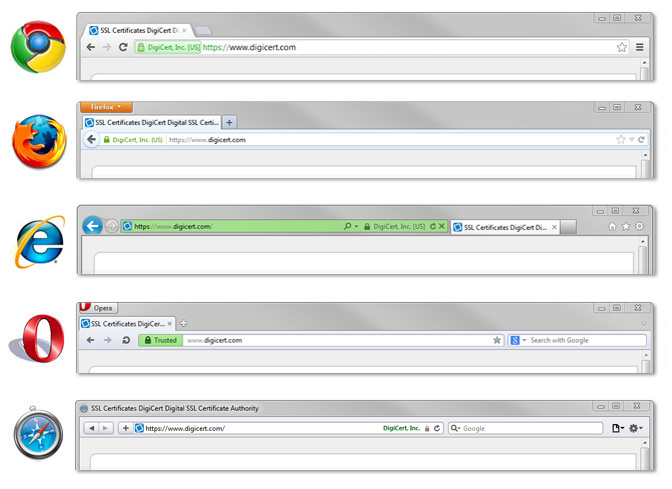
\includegraphics[width=0.60\textwidth]{browservisualq}
  \end{center}
	\vspace{-15pt}
  \caption{Visual cues\cite{browservisualcues}}
\end{wrapfigure}

\subsubsection{Advantages}
The use of internet has drastically increased over the years and so has the different uses of the internet. This has demanded a huge increase in internet security.
As a result of this the use of SSL and TLS has become very popular and quite normal. Even though these security protocols are used all over the internet, it's still a topic almost nobody got any knowledge of. So how does SSL help a website if the users don't know how it works, or what it does? Well, the whole SSL certificate system is built around trust. The only thing the users/customers have to know, is that if a website is secures with SSL, it means that it is safe to use that website. Since the most important part for a website is to show the users that it is in fact safe to use, the universal symbol of safety, a lock, or the color green is added to the address bar of any website that has a valid SSL certificate, as seen in figure 3. 
This ensures the users that a certificate authority, or CA for short,  has reviewed the website and made it safe to use and can be trusted. \cite{digicert}\\
But why is it so important for a company's and websites to have the users trust them? 
The media has for the last couple of years focused a lot on internet security. Because of this more and more people are aware of the risk they take when sending information over the internet. And if they can ensure their users that it is in fact safe, then it is more likely that the user will use the services on their website.\\
Another important advantage for a company to have a SSL certificate is that it reduces the amount of successful phishing sites. This is because it is very difficult for criminals to get a valid SSL certificate on their phishing site.\cite{sslshopper}\\

\subsubsection{Disadvantages}
Even though there are a lot of advantages with using SSL, there are also a couple of disadvantages that companies have to consider before getting a SSL certificate. One of the biggest disadvantages is the fact that getting a SSL certificate can be quite costly. This is because SSL providers have to ensure that their customer's website is secured and validate their identity. And since most companies buy SSL certificates to get more customers and earn more money, it might not be worth getting because of the implementation cost. \cite{sslshopper}\\
Another disadvantage is the fact that encrypting the information takes more resources, and decreases the server performance. Even though this decrease in performance is minimal, it might cause trouble for sites with a lot of traffic. There is also special hardware that can minimize the performance decrease, but that might again not be very cost efficient for the company.  \cite{sslshopper}
